%\documentclass[oribibl]{llncs}
\documentclass[a4paper]{report}
\usepackage{wrapfig}
\usepackage{times}
\usepackage{stmaryrd, latexsym, amsmath, amssymb, wasysym}
\usepackage{fancyvrb}
\usepackage[Lenny]{fncychap}
\usepackage{listings}
\usepackage{url}
\usepackage{semantic}
\usepackage{caption}
\usepackage{array}
\usepackage{graphicx}
\newcommand{\nametklass}{taint-aware }
\newcommand{\nameTklass}{Taint-aware }
\newcommand{\namefunc}{taint-aware }
\newcommand{\suggestions}{Suggestions for lunch \texttrademark }

\newcommand{\arrowop}[1]{$#1\negthickspace #1\negthickspace #1$}
\newcommand{\co}[1]{$\cod{#1}$}
% security type with index
\newcommand{\sts}[1]{s_{#1}^l}
% security type without index
\newcommand{\st}{s^l}
% symbol of constraint IS
\newcommand{\is}{\sim}
% symbol of gconstraint
\newcommand{\guard}{\lhd}
\newcommand{\sleql}{\LHD}
\newcommand{\lleqs}{\preceq}
% tag constraint
\newcommand{\tagup}{\uparrow}
% declassification constraint
\newcommand{\decl}{\downarrow}
% lifting function
\newcommand{\lift}{\nearrow}
% basic type without index
\newcommand{\typ}{\tau}
% basic type with index
\newcommand{\typn}[1]{\tau_{#1}}
% result of type system
\newcommand{\res}[2]{{#1}\mid {#2}}


%\newenvironment{code}{\begin{Verbatim}[fontsize=\footnotesize]}{\end{Verbatim}}

\pagestyle{plain}

\title{A library for Taint Analysis in Python: discussions and implementation}

\newcommand{\myTitle}{A library for Taint Analysis in Python: discussions and implementation}
\newcommand{\mySubtitle}{}
\newcommand{\myAuthor}{Ing. Juan Jos\'{e} Conti}
%\institute{
%Department of Computer Science,
%Chalmers University of Technology\\
%412 96 G\"{o}teborg, Sweden
%}

\author{Juan Jos\'{e} Conti}

\begin{document}

\pagestyle{plain}
\pagenumbering{roman}

%\maketitle
\thispagestyle{empty}

\clearpage
\par\vskip 2cm
\begin{center}
{\Huge\bf \myTitle                                         %PERSONALIZE
\vskip 1cm \Large \mySubtitle                              }           %PERSONALIZE
\par\vspace {6cm}
{\large Graduate Thesis }
\par\vspace {1cm}
{\large ????????????????????\\
%at \\
UTN  }
\par \vspace{1cm}
{\large September 2010  }            %PERSONALIZE
\par\vspace {1cm} {\large by}
\par \vspace {1cm}
{\Large \myAuthor            }                                  %PERSONALIZE
\par\vspace {1cm}
{\large Santa Fe, Argentina}                 %PERSONALIZE
\end{center}

\clearpage

\thispagestyle{empty}
\noindent
Supervisor: Dr. Alejandro Russo \\
Department of Computer Science and Engineering \\
Chalmers University of Technology \\
SE - 412 96 G\"{o}teborg, Sweden \\

\noindent
Co-supervisor: Ms. Susana Romaniz\\
Facultad Regional Santa Fe \\
Universidad Tecnol\'{o}gica Nacional \\
Argentina\\

\vfill\noindent
Copyright \copyright\ 2010 by \myAuthor \\
E-mail: jjconti@frsf.utn.edu.ar

\clearpage

\tableofcontents

\listoffigures
\addcontentsline{toc}{chapter}{List of Figures}

\listoftables
\addcontentsline{toc}{chapter}{List of Tables}

\chapter*{Abstract}
\addcontentsline{toc}{chapter}{Abstract}


Vulnerabilities in web applications present threats to on-line systems.
SQL injection and cross-site scripting attacks are among the
most common threats found nowadays. These attacks are
often result of improper or none input validation. 
To help discover such vulnerabilities, 
popular web scripting 
languages like Perl, Ruby, PHP, 
and Python perform taint analysis.
The analysis is usually implemented using an static (e.g. type
systems) or dynamic (e.g. execution monitors) techniques. 
In the latter case, the Perl, Ruby, PHP, and Python interpreters have
been adapted to provide a taint mode. 
However, modifying interpreters might be a major task in its own
right. In fact, it is very probably that  
new releases of interpreters require to 
be adapted to provide a taint mode.
Differently from previous approaches, 
we show how to provide taint analysis for Python via a library
 written entirely in Python, and thus avoiding modifications in the interpreter.
The concepts of classes, decorators and dynamic dispatch
makes our solution lightweight, easy to use, and particularly neat.
With minimal or none effort, the library can be adapted
to work with different Python interpreters.



\chapter*{Acknowledgement}
\addcontentsline{toc}{chapter}{Acknowledgments}

This work wouldn't be possible without kindly support from many people.

First of all, I would like to express my immense gratitude to my dear supervisor, 
Dr. John Hughes, who has suggested me such an exciting topic, has provided me brilliant ideas
when I met difficulties, and has given me insightful advice as well as zealous encouragement.
I cannot overstate my grateful to Alejandro Russo. This work wouldn't look like it is today
without his clever ideas, enthusiastic discussions, and helpful comments.
Every meeting with them is informative and enjoyable for me.  
I learn a lot not only from their professional expertise but also from their optimistic personalities
when facing problems.
Working with them is definitely an unforgettable experience in my life.

I would like to thank Dr. David Sands, Dr. Andrei Sabelfeld, Aslan Askarov, and people in the Multi
Group at Department of Computer Science and Engineering for providing useful comments on many 
parts of this work. I also like to thank B\"{o}rje Johansson for helping me facilitate the 
whole process.

I want to dedicate this work to my dearest family: my grand mother, Cho-she Tsai, who always fully supports
me since I was a child, my father, Cheng-chih Tsai, and my mother, Li-ching Chao, who encourage me
to pursue my dream and support me with infinite love, and my brother, Yu-chung Tsai, with whom I learn, play, 
and grow. I am also grateful to my lovely relatives whose constantly care and greetings make me
feel warm even in the cold winter of Sweden.

I cannot continue without thanking a group of extraordinary friends. They are Li-ting Chao, 
Chien-chih Chen, Chien-huei Chen, Fei-neng Chuang, Yu-ting Liao, Yueh-ting Liao as well as
other members of NCTU Europe. We share the happiness and the bitterness of studying in Sweden and
strive for graduation together. I will miss our wonderful weekly parties and movie nights.

In the end, I like to express my gratitude to all my friends in Taiwan for helping me
in every aspect and making me feel connected despite far from home.
In particular, I would like to thank Cheng-dar Li, Yi-tzu Lin, and Fu-kuo Tseng.


{\small{
\paragraph{Acknowledgments}
Thanks are due to Arnar Birgisson for interesting discussions.
This work was funded by the Swedish research agencies VR and 
the scholarship program for graduated students 
from the Universidad Tecnol\'{o}gica Nacional, Facultad Regional Santa Fe. 
}}

% real report begins
\cleardoublepage
\pagestyle{plain}
\pagenumbering{arabic}

%%%%%%%%%%%%%%%%%%%%%%%%%%%%%%%%%%%%%%%%%%%%%%%%%%%
%%% 1 INTRODUCTION %%%%%%%%%%%%%%%%%%%%%%%%%%%%%%%%
%%%%%%%%%%%%%%%%%%%%%%%%%%%%%%%%%%%%%%%%%%%%%%%%%%%

\chapter{Introduction}
\label{Chap:Introduction}
%\subimport{01-Introduction}{intro.tex}
In this chapter we introduce the problem  we are facing,
coment traditional ways to solve it,
define the context where we'll be working, which is given by
a particular programming language,
and explain how the thesis is organized.

\section*{The problem of security}
%% Situation: web applications widely use and no security still
Over the past years, there has been a significant increase 
on the number of activities performed on-line.
Users can do almost everything  
using a web browser (e.g. 
watching videos, listening to music, banking, booking flights, planing 
trips and more). Considering the size of Internet and its number of users, 
web applications are probably among the most used pieces of
software nowadays.

Despite its wide use, web applications suffer 
from vulnerabilities that permit attackers to 
steal confidential data, break integrity of systems, 
and affect availability of services. 
When development of web applications is done 
with little or no security in mind,  
the presence of security holes increases dramatically.
%% JJ
Deliver the software on time, pressure for adding new features
instead of fixing bugs and 
%clients paying for what they actually can see,
bad paid jobs,
led most of web developers to don't worry about security.
%%
Web-based vulnerabilities have already  
outplaced those of all other platforms 
\cite{StateWebSecurity} 
and there are 
no reasons to think that this tendency has changed
\cite{FFAWebSecurity}.
%%JJ
Attack a web application is much more easy than attack 
desktop applications, where the attacker needs domain specific knowledge,
or attack the operating system, where the attacker needs low level knowledge.
\cite{StateWebSecurity}
%%


%% Top attacks
According to OWASP \cite{OWASP:Top10:2010}, 
cross-site scripting (XSS) and different kind of injections, like
SQL injection (SQLI), attacks are among 
the most common vulnerabilities on web applications.
Although these attacks are classified differently, they are produced 
by the same 
reason: \emph{user supplied data is sent to sensitive sinks 
without a proper sanitation}.
For example, 
when a SQL query is constructed using an unsanitize string provided by a user, 
SQL injection attacks are likely to occur.
%% mas SQLI? algo de XSS?
%%JJ
%The consequences of these kind of attacks can vary, for example:
Possible consequences of these kind of attacks include:

\begin{enumerate}
\item Impersonate: when an attacker stills the identity of a user
in in web site.
\item Compromise confidential data: when an unauthorized user
reaches data h
e wasn't suppose to reach.
\item Denial of Service: when a resource is not available
to its genuine users.
\item Data destruction.
\end{enumerate}

So the attacker goal is to craft input data to gain some
control over certain operations.
It's important to mention here that the attacker has no
control over the executed code,
just over the input data.

There are different scenarios and different sensitive sinks
where an attacker can act.
%%% Agregar un cuadradito con una deficinion de sskink?
The attacker can  manipulate the data that will be use
to produce an SQL query
and obtain some secret information,
make an operating system injection and execute
arbitrary commands on it or exploit an XSS Vulnerability
and stole a user's credentials
in some web site.
%%

\section*{Taint analysis}
To harden applications against these attacks, 
the implementations of some popular web scripting languages 
%(Perl, Ruby, PHP,  and Python) 
perform taint analysis in a form 
of execution monitors \cite{Perl,Ruby}. In that manner,
not only run interpreters code, but they also perform
security checks.
%Taint analysis can be performed in two ways. Dynamic or static.
Dynamic analysis is usually implemented as a monitor and have the advantage
to produce less false alarms that static analysis. Its main drawbacks are
the overhead produced (because the program and the monitor
runs at the same time)
and the need to modify the interpreter in order to
achieve the desire behavior.

Taint analysis can also be provided through static analysis
\cite{WebSSARI,Jovanovic06pixy:a}. 
This technique produce no overhead because it analyze
the text of the program without need to run it
and no modification of the interpreter is needed.
A mayor disadvantage is that they usually generate
more false alarms than monitors
\cite{Sabelfeld:Russo:PSI09}. 

%Nevertheless, execution monitors usually produce
%less false alarms 
%than traditional static techniques
In other words, 
execution monitors are likely to be more precise
than traditional static techniques. 
In particular, static techniques cannot  
deal with dynamic code evaluation,
a common feature present in web
scripting languages,  
without being too conservative.
Most of the modern web scripting 
languages are capable to dynamically execute code. 
In this thesis, we focus on dynamic techniques.

\section{Introducing \suggestions}
\label{Sec:Suggestions}

We present an example to motivate the use of 
taint analysis in order to discover and repair 
vulnerabilities.

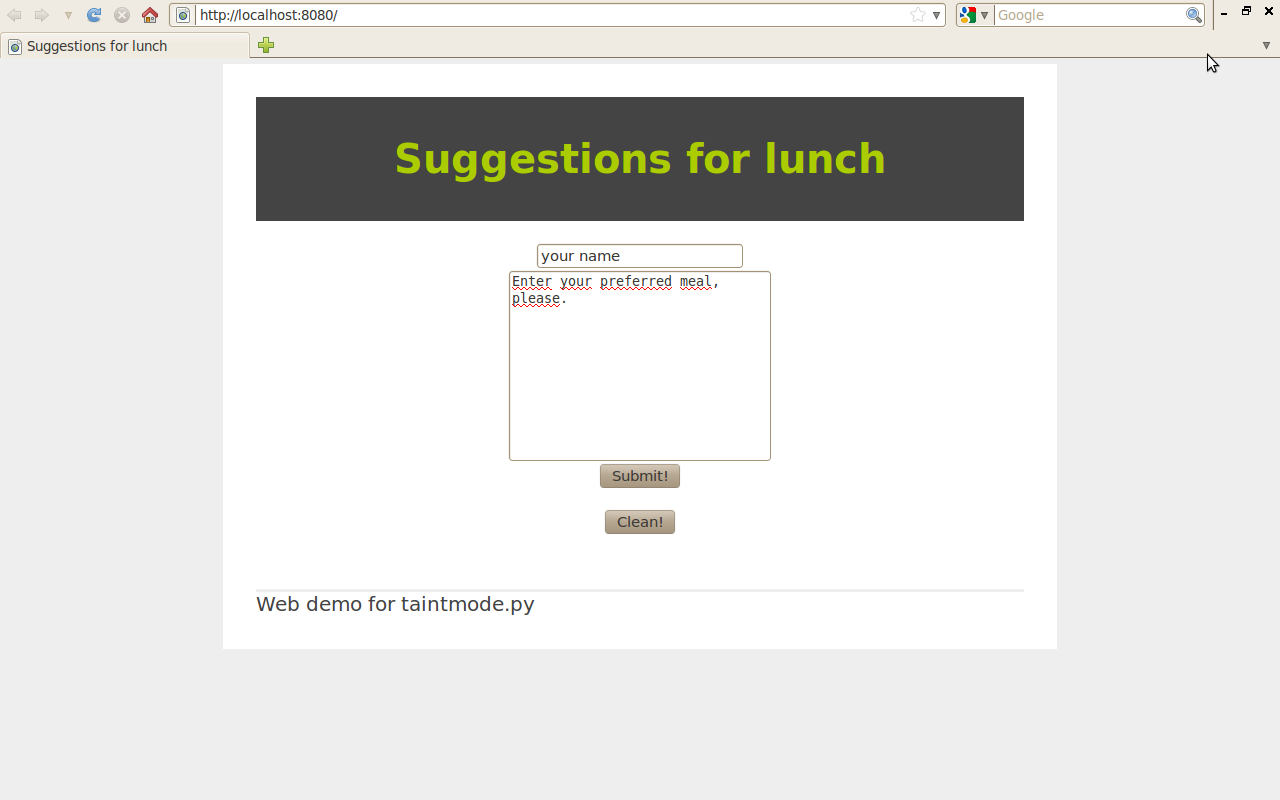
\includegraphics[width=100mm]{lunch1.png}

\suggestions is a web application supposed
to be used in an office to decide what to eat at lunch.
In the morning the employees submit theier suggestion and each day
the designed buyer check the suggestions before go to buy the food.

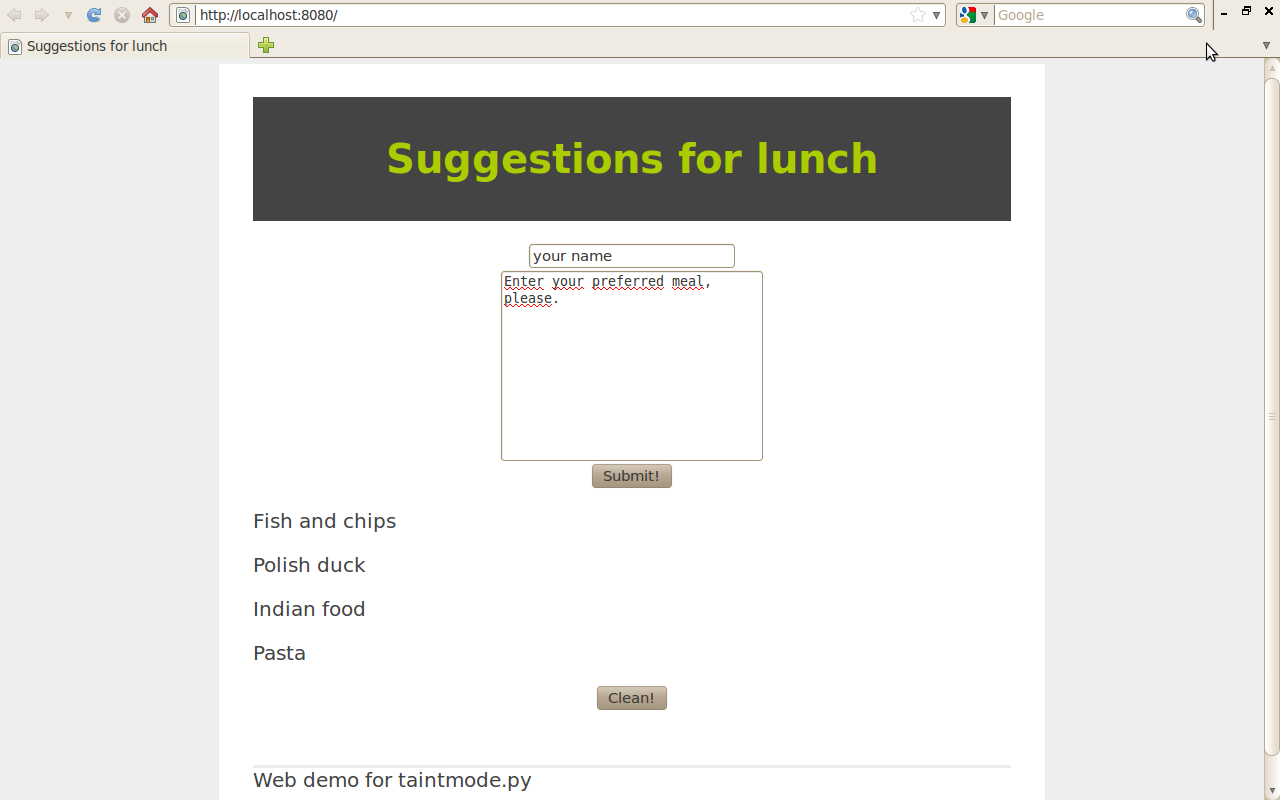
\includegraphics[width=100mm]{lunch2.png}

It seems to work prety well, but the application have a problem. It uses
as datastore a text file and use operating system facilities in order to
store de information in the file.

%\begin{wrapfigure}{c}{6.5cm}
\begin{figure}[h]
%\vspace{-25pt}
{\small{
\lstinputlisting[language=Python,numbers=left]
{lunchproblem.py}
\caption{\label{fig:example}A problem in the web application}
}}
%\vspace{-15pt}
\end{figure}
%\end{wrapfigure}


We can see that data received from the untrusted source
\texttt{web.input} is used
with no validation to build a command tha later is used
in the sensitive sink \texttt{os.system}. 
\texttt{os.system} is a Python object that let the 
programmer execute raw commands against the operating system.

\subsection*{Attacks} % va la subseccion?
\label{Sec:Attacks}
An attacker can abuse this application in order to perform different attacks.
Instead of supply his desire meal, he can submit \texttt{; ls} to make the 
executed command list the files in the application root directory and save that
list in the suggestions file:

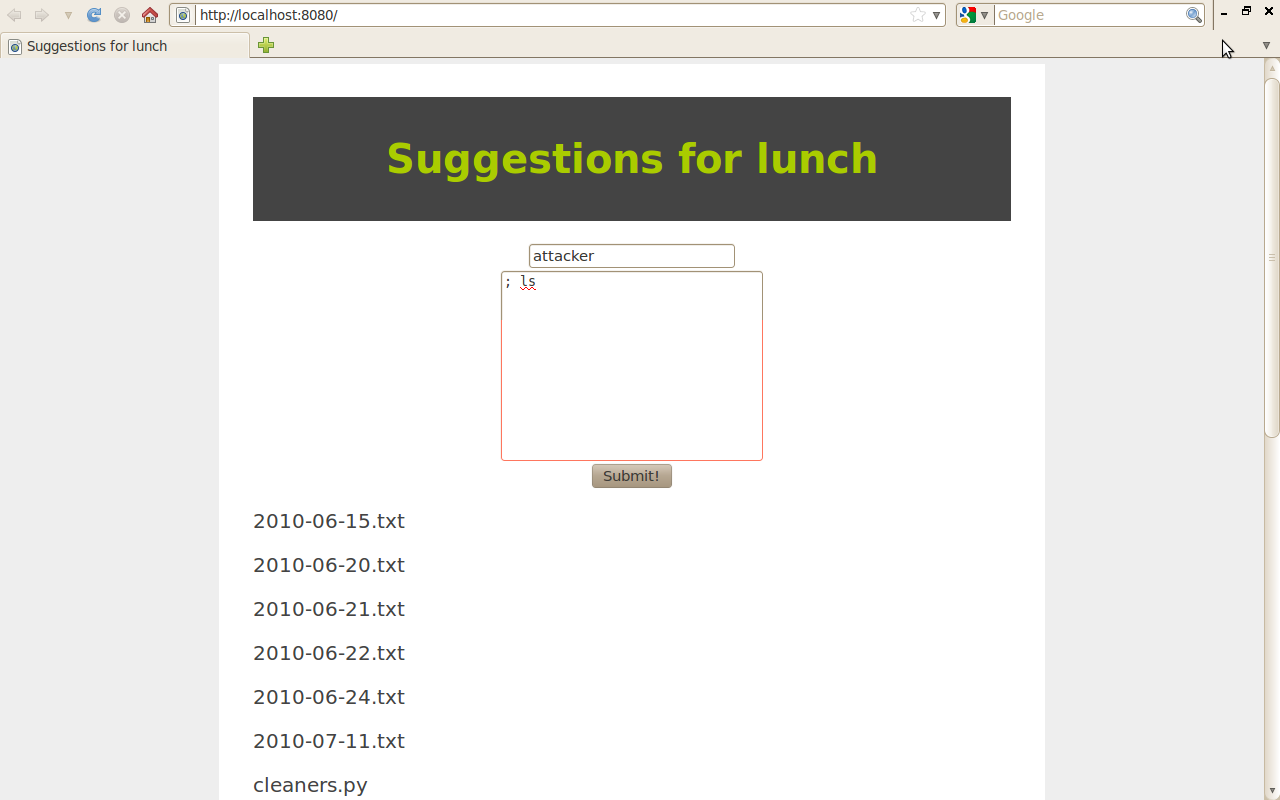
\includegraphics[width=100mm]{lunch3.png}

If he find something instresting, for example a file called 
\texttt{passwords.txt},
he can submit \texttt{; cat passwords.txt}
and read the content of that file:

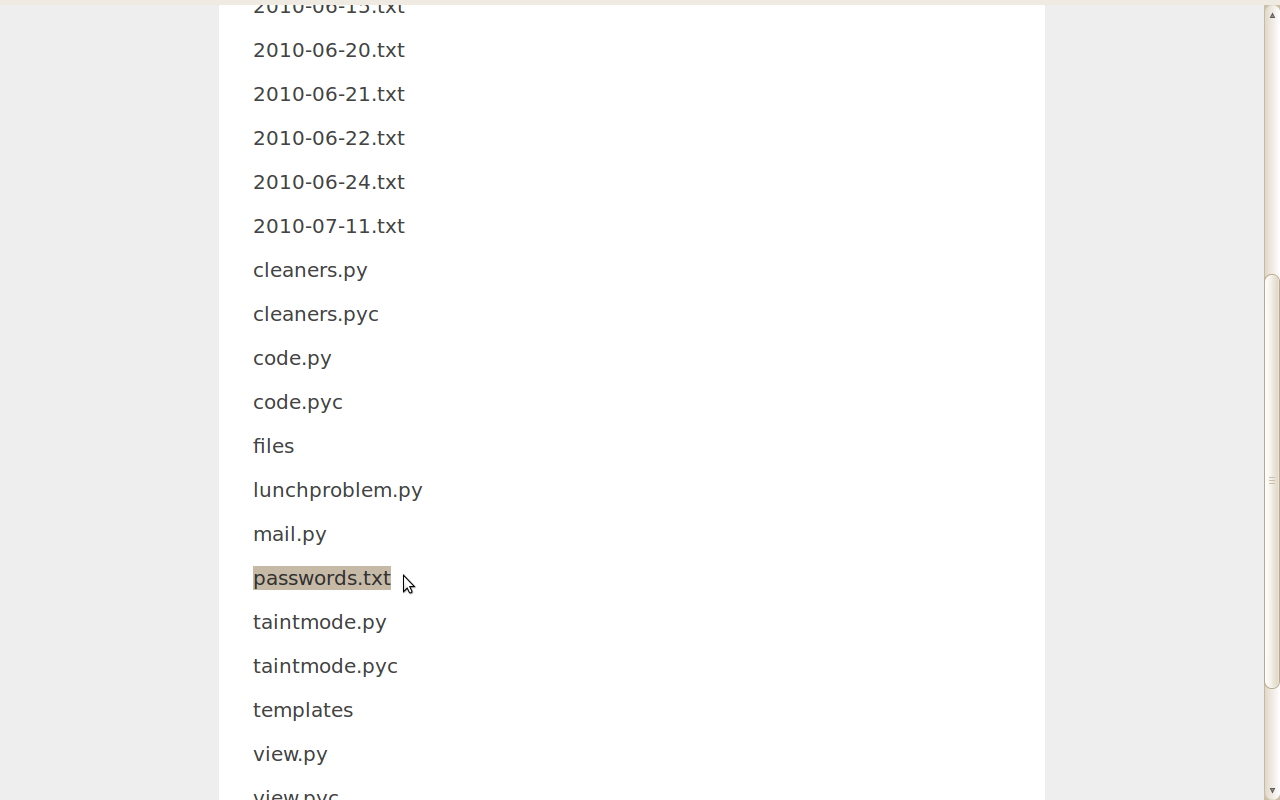
\includegraphics[width=100mm]{lunch4.png}

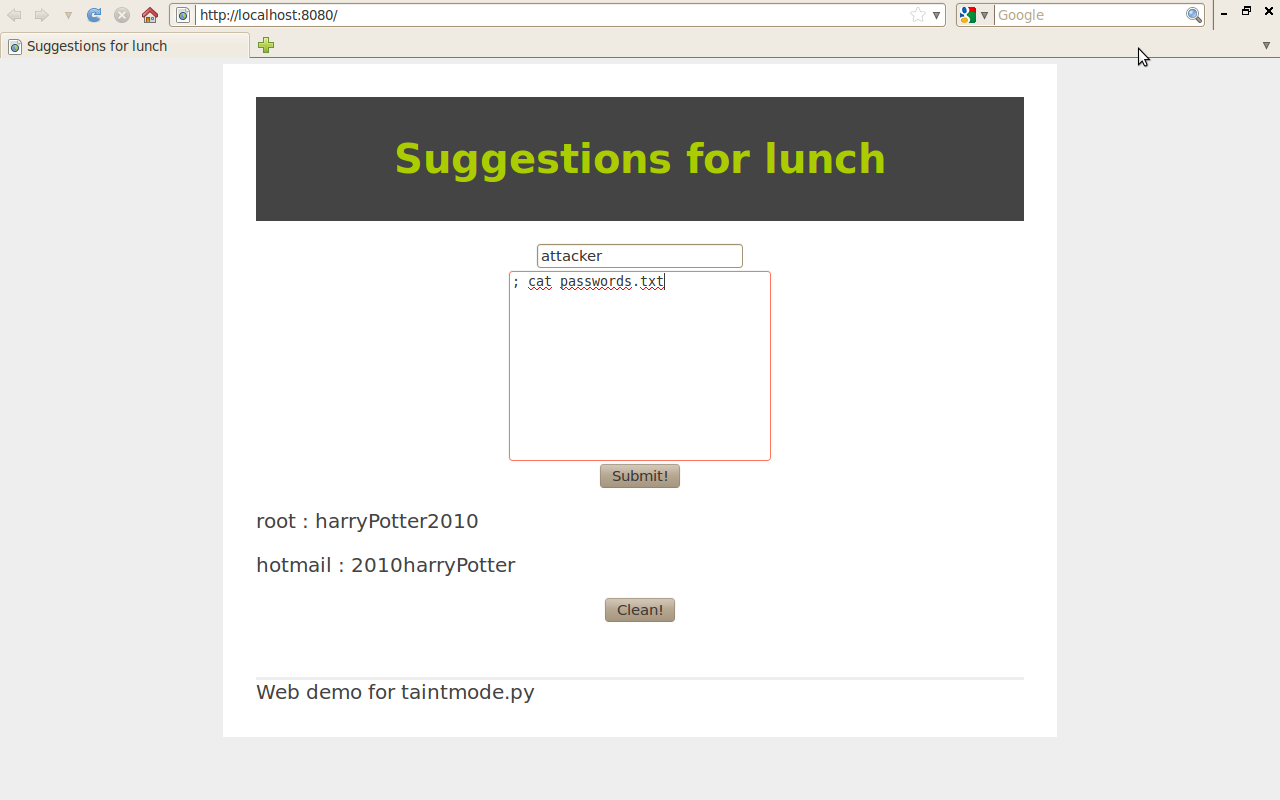
\includegraphics[width=100mm]{lunch5.png}

Even more, he can read the content of system sensitive files and,
for example, submitting \texttt{; cat /etc/passwd} get the list
of the system users:

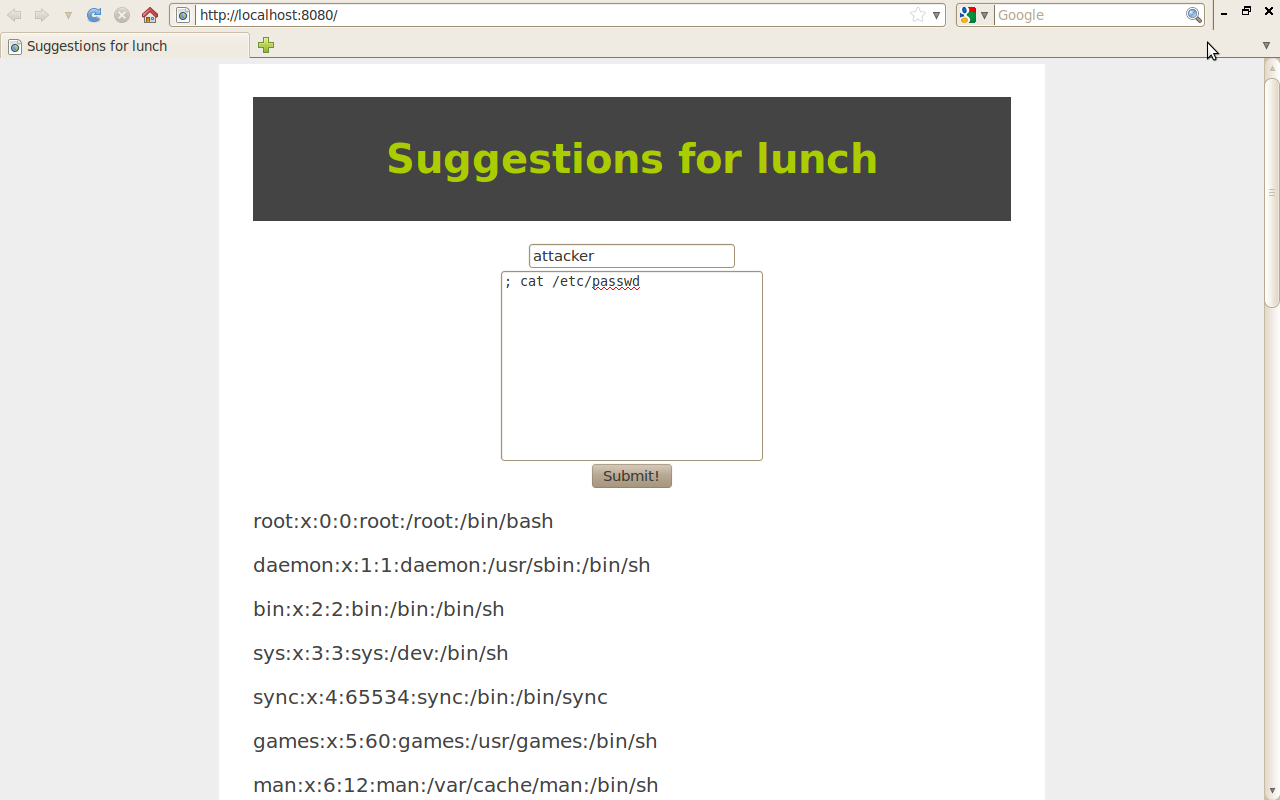
\includegraphics[width=100mm]{lunch6.png}


These attacks demonstrate how, 
what was intended to be a simple web application,  
can become a web-based file browser or a terminal. To avoid 
these vulnerabilities, applications need to rigorously check 
for malicious data provided by users or any other 
untrustworthy source. 

Taint analysis helps to detect when 
data is not sanitize before it is used on security critical 
operations. In Chapter \ref{Chap:Library}, we show how to harden 
\suggestions in order to reject the vulnerabilities 
shown in Section Attacks.

\section{Python programming language}

As its web site explains\cite{Python},
%Python is a programming language that lets programmers
%work more quickly and integrate their systems more effectively.
%Once Python is lerned gains in productivity
%and lower maintenance costs are inmidiatly seen.
Python is an interpreted, interactive, object-oriented programming language.
It incorporates modules, exceptions, dynamic typing, 
very high level dynamic data types, and classes. 
Python combines remarkable power with very clear syntax. 
It has interfaces to many system calls and libraries, as well 
as to various window systems, and is extensible in C or C++. 
It is also usable as an extension language for applications that 
need a programmable interface. Finally, Python is portable: it 
runs on many Unix variants, on the Mac, and on PCs under 
MS-DOS, Windows, Windows NT, and OS/2.

We said that the common way of implement taint mode in a programming
language is modifying the interpreter. Rather than doing this,
we present how to provide
a taint mode for Python via a library written entirely in Python. 

Python is spreading fast inside
web development \cite{WikiPython}. 
For instance, 
the popular Wiki engine 
MoinMoin (e.g. used by Ubuntu forums)
and Youtube are mostly written in Python.  Among companies, 
we can mention Google, which uses 
the language for some of its search-engine internals at
Google Groups, Gmail, and Google Maps.
There are also many numbers of web development frameworks written
in Python; Django\cite{Django}, de most popular one is widely used
in the industry and was addopted as one of the first supported
tools in Google App Engine cloud computing platform.

Besides its successful use, Python presents 
some programming languages abstractions that makes possible 
to provide a taint mode via a library. For example, 
Python decorators \cite{Lutz:1999:LP} are a non-invasive and simple 
manner to declare sources of tainted data, sensitive sinks, and 
sanitation functions. Python's 
object-oriented and dynamic typing mechanisms allows the 
execution of the taint analysis with almost no modifications in the
source code. 

The library provides a general method to enhance Python's built-in
classes with tainted values. 
%To demostrate the flexibility of our approach, 
%the library enhances the built-in classes for
%strings, integers, and floats. 
In general, taint
analysis tends to only consider strings or characters 
\cite{Perl,Nguyen05,Haldar05dynamictaint,KozlovPetukhov07,Futo07,SeoLam2010}.
% when 
%implemented as part of interpreters. 
In contrast, our library 
can be easily adapted to consider different built-in
classes
% as well as users' specific ones, 
and thus providing a taint
analysis for a wider set of data types. 
By only considering tainted strings, the library provides 
a similar analysis than in \cite{KozlovPetukhov07},
but without modifying the Python interpreter.
To the best of our knowledge, a
library for taint analysis has not been considered before. 

\section{Organization}
The rest of the thesis is organized as following. Chapter 2 describes background
knowledge, existing approaches for taint mode and the general idea of tain analysis.
Chapter 3 introduces the library, its API and shows how to use it to harden
the example application \suggestions.
Chapter 4 presents implementation details of the library with special attention
to those Python features that make it easy to build this technology in a
noninvasive way from the programmer point of view.
Chapter 5 explains limitations of the current approach and discusses alternatives.
In Chapter 6 we present conclusions and ideas for future works.
library source code as well as the example source code are provided in the Appendix.




%%%%%%%%%%%%%%%%%%%%%%%%%%%%%%%%%%%%%%%%%%%%%%%%%%%
%%% 2 Taint Analysis %%%%%%%%%%%%%%%%%%%%%%%%%%%%%%
%%%%%%%%%%%%%%%%%%%%%%%%%%%%%%%%%%%%%%%%%%%%%%%%%%%

\chapter{Taint Analysis in general + related works}
\label{Chap:taint}
A way to face these problems is using Taint Analysis. Usually enforcesd 

Data received from a client is considerer tainted. We can't trust in data from the outside because we don't know who generate it. May be a real user, maybe an attacker or even an attacker program. 

Tainted data can be untainted by a sanitization process.

We don't want tainted data to reach sensitive sinks.

In the image you can see different sanitization processes represented with different colors. This means that data that will finish in different sinks needs to be properly cleaned for that kind of sink.

It's not the same the function you'll use to protect a page renderer against XSS than the DB against SQLI.

% Taint analsys
%A 
Taint analysis is an automatic approach to find vulnerabilities.
Intuitively, taint analysis restricts how tainted or untrustworthy 
data flow inside programs. Specifically, it constrains data 
to be untainted (trustworthy) 
or previously sanitized when 
reaching sensitive sinks. 
%In a web scenario, 
%user input is frequently considered as tainted, while 
%HTTP-request, SQL queries, and other security critical operations 
%are classified as sensitive sinks. 
Perl was the first scripting 
language to provide taint analysis 
as an special mode of the  
interpreter called \emph{taint mode} \cite{BekmanCholet2003}. 
Similar to Perl, some interpreters for 
 Ruby \cite{thomas2004prub}, PHP \cite{Nguyen05}, and 
recently Python \cite{KozlovPetukhov07} have been 
carefully modified to provide taint modes.
Adapting interpreters to incorporate taint analysis 
present two major drawbacks that directly 
impact on the adoption of this technology. 
Firstly, incorporating taint analysis into an interpreter 
might be a major task in its own right. Secondly, it is 
very probably that it is necessary to repeatedly adapt an  
interpreter at every new version or release of it.


\begin{wrapfigure}{r}{6.5cm}
%\begin{figure}[t]
\vspace{-25pt}
{\small{
\lstinputlisting[language=Python,numbers=right, numberstyle=\tiny]{email.py}
\caption{\label{fig:example}Code for \texttt{email.py}}
}}
\vspace{-15pt}
%\end{figure}
\end{wrapfigure}
%%% Solution / Contributions
Rather than modifying interpreters, we present how to provide
a taint mode for Python via a library written entirely in Python. 
Python is spreading fast inside
web development \cite{WikiPython}. 
%For instance, 
%the popular Wiki engine 
%MoinMoin (e.g. used by Ubuntu forums)
%and Youtube are mostly written in Python.  Among companies, 
%we can mention Google, which uses 
%the language for some of its search-engine internals at
%Google Groups, Gmail, and Google Maps.
Besides its successful use, Python presents 
some programming languages abstractions that makes possible 
to provide a taint mode via a library. For example, 
Python decorators \cite{Lutz:1999:LP} are a non-invasive and simple 
manner to declare sources of tainted data, sensitive sinks, and 
sanitation functions. Python's 
object-oriented and dynamic typing mechanisms allows the 
execution of the taint analysis with almost no modifications in the
source code. 
%\marginpar{Check later what about decorating Bool} 


The library provides a general method to enhance Python's built-in
classes with tainted values. 
%To demostrate the flexibility of our approach, 
%the library enhances the built-in classes for
%strings, integers, and floats. 
In general, taint
analysis tends to only consider strings or characters 
\cite{Perl,Nguyen05,Haldar05dynamictaint,KozlovPetukhov07,Futo07,SeoLam2010}.
% when 
%implemented as part of interpreters. 
In contrast, our library 
can be easily adapted to consider different built-in
classes
% as well as users' specific ones, 
and thus providing a taint
analysis for a wider set of data types. 
By only considering tainted strings, the library provides 
a similar analysis than in \cite{KozlovPetukhov07},
but without modifying the Python interpreter.
To the best of our knowledge, a
library for taint analysis has not been considered before. 

\section{Related work}


%%%%%%%%%%%%%%%%%%%%%%%%%%%%%%%%%%%%%%%%%%%%%%%%%%%
%%% 3 A library for Taint Analysis in Python %%%%%%
%%%%%%%%%%%%%%%%%%%%%%%%%%%%%%%%%%%%%%%%%%%%%%%%%%%
\chapter{A library for Taint Analysis in Python}
\label{Chap:Library}
In this chapter we review \texttt{taintmode.py}, a library
presented orinally in \cite{PythonLib}. After some words on the 
subject of implicit flows, wich are not covered by the library,
we'll show simple examples of use, more elavorated API examples
and finally we'll apply the library to \suggestions, the application
example introduced in \ref{Chap:Introduction}.

\section*{Implicit flows}

\begin{figure}[t]
{\small{
\begin{minipage}[t]{0.5\linewidth}
\lstinputlisting[language=Python,numbers=left,numberstyle=\tiny]{implicit.py} 
\end{minipage}
\caption{\label{fig:implicit}An implicit flow}
}}
\end{figure}

On most situations, taint analysis \cite{Perl,Ruby} 
propagates taint information on assignments.  
Intuitively, when the right-hand side of an assignment uses a tainted value, 
the variable appearing on the left-hand side becomes tainted.
Taint analysis can be seen as an information-flow tracking 
mechanism for integrity \cite{Sabelfeld:Myers:JSAC}. 
In fact, taint analysis is just a mechanism to 
track explicit flows, i.e. direct flows of information 
from one variable to another. 
Taint analysis tends to ignore 
implicit flows \cite{Denning:Denning:Certification}, i.e. 
flows through the control-flow constructs of the language. 

Figure \ref{fig:implicit} presents an implicit 
flow. Variables \texttt{t} and \texttt{u} are 
tainted and untainted, respectively.
Observe that variable \texttt{u} 
is untainted after the execution of the branch since 
an untainted value ($\texttt{'a'}$ or
$\texttt{''}$) is assigned to it. Yet, the value of the tainted variable 
$\texttt{t}$ is copied into the untainted variable 
\texttt{u} when \texttt{t == 'a'}. 
% REVER SI DEJO ESTE EJEMPLO O UNO MAS PYTHONICO
It is not difficult to imagine 
programs that circumvent the taint analysis by
copying the content of tainted strings 
into untainted ones by using implicit flows\cite{Russo:IOS}.

In scenarios where attackers has full control over the code 
(e.g. when the code is potentially malicious), implicit flows present
an effective way to circumvent the taint
analysis. In this case, the attackers' goal  is to craft the code and input 
data in order to circumvent security mechanisms. There is a large body
of literature on the area of language-based security regarding 
how to track implicit flows \cite{Sabelfeld:Myers:JSAC}. 


In the other hand, there're scenarios where 
the code is non-malicious, i.e. written without malice. 
Despite the good intentions and experience of programmers, 
the code might still contain vulnerabilities 
as the ones
described in Section \ref{sec:example}. The attackers' goal  
consists on craft input data in order to exploit 
vulnerabilities and/or corrupt data. In this scenario,
taint analysis certainly helps to discover vulnerabilities. 

How dangerous are implicit flows in non-malicious code? We argue that they
are frequently harmless \cite{Russo:IOS}. The reason for that 
relies on that non-malicious programmers
need to write a more involved, and rather unnatural,
code in order to, for instance, copy tainted strings into untainted ones. 
In contrast, to produce explicit flows, programmers simply
need to forget a call to some sanitization function. 
In this work, we consider 
scenarios where the analyzed code is non-malicious. 



\section{Using the library}

\subsection*{Tags}

By default, tags can take values  
\texttt{XSS}, \texttt{SQLI}, \texttt{OSI} (Operating System Injection), and
\texttt{II} (Interpreter Injection).
These values are used to indicate specific vulnerabilities that 
could be exploited by tainted data.
For instance, 
tainted data associated with tag \texttt{SQLI} is likely to exploit 
SQL injection vulnerabilities.

\subsection*{API Examples}
This section %of
includes examples of the key concepts handled by the library,
which are the key concepts of the whole Taint Analysis idea:

\begin{enumerate}
\item Untrusted sources: from wich untrusted values arrives to the program.
\item Cleaner functions: used to sanitizes untrusted values into trusted ones.
\item Sensitive sinks: places where we don't want utrusted values to arrive.
\end{enumerate}

The examples are capures of an interactive session in 
the Python's REPL\footnote{Read-Eval-Print-Loop}. % SALE AL PIE?

\subsection*{The \texttt{taint} primitive}

\texttt{taint(o, v=None)}

\texttt{taint} is a helper function for taint
the value o with the vulnerability v.

If v is not provided, taint with all types of taints.

\begin{figure}[t]
{\small{
\begin{minipage}[t]{0.5\linewidth}
\lstinputlisting[language=Python,numbers=left,numberstyle=\tiny]{ex_taint1.txt} 
\end{minipage}
\caption{\label{fig:taint1}Tainting with all vulnerabilities}
}}
\end{figure}

\begin{figure}[t]
{\small{
\begin{minipage}[t]{0.5\linewidth}
\lstinputlisting[language=Python,numbers=left,numberstyle=\tiny]{ex_taint2.txt} 
\end{minipage}
\caption{\label{fig:taint2}Tainting with Interpreter Injection vulnerability}
}}
\end{figure}

\subsection*{The \texttt{tainted} primitive}

\texttt{tainted(o, v=None)}

\texttt{tainted} tells if a value o is tainted for the given
vulnerability v.

If v is not provided, checks for all taints. If the value is tainted
with at least one vulnerability, returns True.

\begin{figure}[t]
{\small{
\begin{minipage}[t]{0.5\linewidth}
\lstinputlisting[language=Python,numbers=left,numberstyle=\tiny]{ex_tainted.txt} 
\end{minipage}
\caption{\label{fig:taint1}Is a value tainted?}
}}
\end{figure}

\subsection*{How to define an untrusted source?}

The simplest way of marking an input as untrusted, is using the \texttt{untrusted} decorator.
One way to use it is using Python's sintactic sugar for decorators.

\begin{figure}[t]
{\small{
\begin{minipage}[t]{0.5\linewidth}
\lstinputlisting[language=Python,numbers=left,numberstyle=\tiny]{ex_untrusted1.txt} 
\end{minipage}
\caption{\label{fig:untrusted1}An utrusted source using the \texttt{untrusted} decorator}
}}
\end{figure}

In the example, the decorator is applied to the \texttt{values\_from\_outside} function
when it's defined. After this, every time the function is called, the returned value
is tainted with all the vulnerabilities; that is, is marked with all the avaliable tags.

The second way of using the \texttt{untrusted} decorator is through a function call.
This is extremly useful when wanting to mark a function for which we don't have access 
to its definition. For example, marking third party libraries.

\begin{figure}[t]
{\small{
\begin{minipage}[t]{0.5\linewidth}
\lstinputlisting[language=Python,numbers=left,numberstyle=\tiny]{ex_untrusted2.txt} 
\end{minipage}
\caption{\label{fig:untrusted2}An utrusted source using the \texttt{untrusted} decorator as a function call}
}}
\end{figure}

There is a more elavorated use case and it mainly take place when using some frameworks.
We are asked to define a new function or method and the framework is in charge of
calling this function when ever a value from the outside is received.

The \texttt{untrusted\_args} decorator have two arguments. The first one is a list 
of positions and the second one is a list o keywords. In this case, the
positional arguments in the positions list and the keyword arguments in the kwywords
list are the ones that are marked as untrusted, not the returned value.

\begin{figure}[t]
{\small{
\begin{minipage}[t]{0.5\linewidth}
\lstinputlisting[language=Python,numbers=left,numberstyle=\tiny]{ex_untrusted_args.txt} 
\end{minipage}
\caption{\label{fig:untrusted_args}An utrusted source using the \texttt{untrusted\_args} decorator}
}}
\end{figure}

In figure \ref{fig:untrusted_args} the decorator arguments express that positions 1 and 2 ass well
as keyword \texttt{file} will be marked as untrusted whenever the function is executed.

The rest of the code make a function call and capture the result in two variables that are then iterated
in order to show which values are tainetd and which are not. 

\subsection*{How to define a cleaner function?}

\texttt{cleaner(v)}

\texttt{cleaner} is a decorator used to tell that a method or function is able to clean
taints on a value, that is, remove certain vulnerability tag (\texttt{v} argument).

Again, the decorator can be applied using the sintactic sugar provided by the
language or a function call.

In image \ref{fig:cleaner1} a value tainted with \texttt{XSS} is cleaned using
the function plain\_text which was already marked as capable to remove that vulnerability.

\begin{figure}[t]
{\small{
\begin{minipage}[t]{0.5\linewidth}
\lstinputlisting[language=Python,numbers=left,numberstyle=\tiny]{ex_cleaner1.txt} 
\end{minipage}
\caption{\label{fig:cleaner1}A cleaner function}
}}
\end{figure}

There is also a similiar decorator called \texttt{validator}, with a different semantic.

\texttt{validator(v, cond=True, nargs=[], nkwargs=[])}

It mark a function or method as capable to validate its input.

\texttt{nargs} is a list of positions. Positional arguments in that positions are
the ones validated.
\texttt{nkwargs} is a list of keywords. Keyword arguments for those keys are the ones
validated.

\texttt{cond} can be either \texttt{True} or \texttt{False}.
If the decorated function returns cond, tag v will be removed from the the validated
inpunt.

For example, in a function called \texttt{is\_not\_digit}, cond is liked to be False. If
\texttt{is\_not\_digit} returns \texttt{False}, then the value \emph{is} valid and have no craft data
on it. 

\begin{figure}[t]
{\small{
\begin{minipage}[t]{0.5\linewidth}
\lstinputlisting[language=Python,numbers=left,numberstyle=\tiny]{ex_validator2.txt} 
\end{minipage}
\caption{\label{fig:cleaner1}The \texttt{is\_not\_digit} validator}
}}
\end{figure}

For a function called is\_digit, cond is liked to be True.

\begin{figure}[t]
{\small{
\begin{minipage}[t]{0.5\linewidth}
\lstinputlisting[language=Python,numbers=left,numberstyle=\tiny]{ex_validator1.txt} 
\end{minipage}
\caption{\label{fig:cleaner1}The \texttt{is\_digit} validator}
}}
\end{figure}

\subsection*{How to define a sensitive sink?}

\texttt{ssink(v=None, reached=reached)}

\texttt{ssink} marks a function or method as sensitive to tainted data.
If it is called with a value with the v tag (or any tag if v is None),
the decorated function it's not executed and reached is executed instead.

These sinks are sensitive to a kind of vulnerability, and must be specified when
the decorator is used.

\begin{figure}[t]
{\small{
\begin{minipage}[t]{0.5\linewidth}
\lstinputlisting[language=Python,numbers=left,numberstyle=\tiny]{ex_sensitive.txt} 
\end{minipage}
\caption{\label{fig:untrusted}An utrusted source}
}}
\end{figure}

If the sentive function is called with a value tainted with the same vulnerability the sink is
sentive to, then the execution can be cut and a warning message printed explaing what happened.

Calling the function with other values, event tainted, is allowed.

\section{Hardening \suggestions}
\label{sec:securing}

In section \ref{Sec:Suggestions} we introduced \suggestions, a web application used in an
office to organized what to eat each day. We also showed some security problems the application have.

In this section, we'll show hot to use \texttt{taintmode.py} to Hardening \suggestions.

\subsection*{Imports}

The only thing we need to add to the original program are the following lines:

\begin{figure}[t]
{\small{
\begin{minipage}[t]{0.5\linewidth}
\lstinputlisting[language=Python,numbers=left,numberstyle=\tiny]{harden.txt} 
\end{minipage}
\caption{\label{fig:secured} Secure version of \suggestions}
}}
\end{figure}

We import from the \texttt{taintmode} module, mark \texttt{web.input} as a
untrusted soruce, and \texttt{os.system} as a sensitive sink to Operating System Injection (\texttt{OSI}).
Finally, we execute \texttt{taintmode.ends\_execution()} in order to explicitly say that we want the
execution to be cut when ever a problem occurs.

If now, we try to submit some data into the application form, we'll see that nothing happens. Nothing?
We don't see anything new in the web page because the execution was cut. If we see the log files of the 
application, we'll find something like \ref{fig:error}

\begin{figure}[t]
{\small{
\begin{minipage}[t]{0.5\linewidth}
\lstinputlisting[]{harden_error.txt} 
\end{minipage}
\caption{\label{fig:securederror} \suggestions}
}}
\end{figure}

The input data was harmless, but anyway the execution was cut. A value with an \texttt{OSI}
taint arrived to an \texttt{OSI}-sensitive sink. How do we fix the app in order to make it
useful while it stop attackers? The application needs to use a cleaner function. So we impor it
and mark it as capable to clean data agains \texttt{OSI}:

\begin{figure}[t]
{\small{
\begin{minipage}[t]{0.5\linewidth}
\lstinputlisting[language=Python,numbers=left,numberstyle=\tiny]{harden_cleaner.txt} 
\end{minipage}
\caption{\label{fig:securedcleaner} Import a cleaner}
}}
\end{figure}

The final step is to \emph{use} \texttt{osi\_cleaner} in the code:

\begin{figure}[t]
{\small{
\begin{minipage}[t]{0.5\linewidth}
\lstinputlisting[language=Python,numbers=left,numberstyle=\tiny]{harden_new.txt} 
\end{minipage}
\caption{\label{fig:securednew} Using the cleaner}
}}
\end{figure}

Observe that the added code is minimal and as less intrusive as possible.
% ALGO MAS PARA CERRAR EL CAPITULO?


%%%%%%%%%%%%%%%%%%%%%%%%%%%%%%%%%%%%%%%%%%%%%%%%%%%
%%% 4  Implementation %%%%%%%%%%%%%%%%%%%%%%%%%%%%%
%%%%%%%%%%%%%%%%%%%%%%%%%%%%%%%%%%%%%%%%%%%%%%%%%%%
\chapter{Implementation}
\label{Chap:Implementation}
\begin{figure}[t]
{\small{
\lstinputlisting[language=Python,numbers=left, numberstyle=\tiny]{taint_class.py}
\caption{\label{fig:generate} Function to generate \nametklass classes}
}}
\end{figure}

In this section we present the details of our implementation. Due to lack of
space, we show the most interesting parts.
The full
implementation of the library is publicly available at \cite{PythonLib}.


%% Intuitively classes and methods
One of the core part of the library 
deals with how to keep track of taint information 
for built-in classes.
% and their corresponding operations.
%main challenge that the library implements is how to 
%The core of the library implements how built-in 
%values, and their corresponding operations, can keep track of 
%taint information. 
The library defines 
subclasses of built-in classes
in order to indicate if values are tainted or not.
%(like \texttt{str} or \texttt{int})
An object of these subclasses posses an attribute to indicate a set 
of tags 
%(Section \ref{sec:using}) 
associated to it. 
%When the set of tags is empty, objects are not tainted.
Objects are considered untainted when the
set of tags is empty. 
%Objects are not tainted when its set of tags is the empty.
%In the case that this set is empty, 
%the value is not tainted. 
We refer to these subclasses as
\emph{\nametklass classes}.
In addition, the methods inherited from the built-in classes 
are redefined in order to propagate taint information. 
%This propagation is done by updating the set of tags
%in tainted objects. 
More specifically, methods that belong to 
\nametklass classes return objects with  
the union of tags found in their arguments and 
the object calling the method. 
In Python, 
the dynamic dispatch 
mechanism guarantees that, for instance, 
the concatenations of untainted and tainted strings is performed 
%carried out 
with calls to methods of \nametklass classes, which properly   
%value, from a built-in class, and a tainted value, from its 
%corresponding \nametklass class, results in calls to 
%the methods of the \nametklass class. In that manner, 
%the 
propagates taint information. % can be successfully done. 
% can then be accordingly done.
%We illustrate these ideas later  with
%examples.

\section{Generating \nametklass classes}
\label{sec:general}

%\end{figure}
\begin{wrapfigure}{r}{7.5cm}
\vspace{-30pt}
{\small{
\lstinputlisting[language=Python,numbers=right, numberstyle=\tiny]{propagate.py}
\caption{\label{fig:propagate} Propagation of taint information}
}}
\vspace{-15pt}
\end{wrapfigure}
Figure \ref{fig:generate} presents a function to generate
\nametklass classes. The function takes a built-in
class (\texttt{klass}) and a list of its methods
(\texttt{methods}) where taint propagation 
must be performed. 
%\textbf{DESCRIBE ON THIS SENTENCE
%WHY NOT GENERAL INSTEAD OF A LIST OF METHODS}. 
Line 2 defines the name of the \nametklass class \texttt{tklass}.
Objects of \texttt{tklass}  
are associated to the empty set
 of tags when created (lines 3--6). Attribute 
\texttt{taints} is introduced to 
indicate the tags related to tainted values.
% to them.
Using Python's introspection features, variable 
\texttt{d} contains, among other
things, the list of methods for the built-in class (line 7). 
For each method in the built-in class and in \texttt{methods} 
(lines 8--10), the code adds to \texttt{tklass} a 
method that has the same name and computes the same results 
but also propagates taint information  
%, where the method 
%also performs propagation of taint information 
(line 11).
%Observe that added methods have the same names as the ones 
%in the built-in class.  
Function \texttt{propagate\_method} is explained below.
Lines 12--15 set method \texttt{\_\_radd\_\_} to taint-aware 
classes when built-in classes do not include that method but 
\texttt{\_\_add\_\_}.
%and not \texttt{\_\_radd\_\_}. 
Method \texttt{\_\_radd\_\_} is called to implement the binary operations 
with reflected (swapped) operands\footnote{The built-in class 
   for strings implements all 
   the reflected versions of its operators but \texttt{\_\_add\_\_}.}. 
%This function is called only if the left operand does not support the 
%corresponding operation. 
For instance, to evaluate the expression \texttt{x+y}, where \texttt{x} is a built-in string 
and y is a taint-aware string, Python calls \texttt{\_\_radd\_\_} from 
\texttt{y} and thus executing \texttt{y.\_\_radd\_\_(x)}. In that manner, 
the taint information of \texttt{y} is propagated to the expression. Otherwise, the method
\texttt{x.\_\_add\_\_(y)} is called instead, 
which results in an untainted string.
Finally, the \nametklass class is returned (line 16). 

The implementation of \texttt{propagate\_method} is shown in Figure
\ref{fig:propagate}. The function takes a method and returns another
method that computes the same results but propagates taint information. Line 3
calls the method received as argument and stores the results in 
\texttt{r}. 
Lines 4--9 collect the tags from the current object and 
the method's arguments into \texttt{t}. 
Variable \texttt{r} 
might refer to an object of a built-in class and
therefore not include the attribute \texttt{taints}. For that reason, 
function \texttt{taint\_aware} is designed to 
transform objects from built-in classes  
into \nametklass ones. 
For example, if \texttt{r} refers
to a list of objects of the class \texttt{str}, function \texttt{taint\_aware} returns  
a list of objects of the \nametklass class 
derived from \texttt{str}. 
Function \texttt{taint\_aware} 
is essentially implemented as a structural mapping on list, tuples,
sets, and dictionaries. 
The library does not
taint built-in containers, but rather their elements. This is a design decision 
based on the assumption that non-malicious code does not exploit
containers to circumvent the taint analysis (e.g. by 
encoding the value of tainted integers into 
the length of lists).
%For instance, we assume that nonmalicious programs do not 
\begin{wrapfigure}{r}{6.6cm}
\vspace{-20pt}
{\small{
\lstinputlisting[language=Python]{factory.py}
\caption{\label{fig:factory} \nameTklass classes for strings and
  integers}
}}
\vspace{-20pt}
\end{wrapfigure}
Otherwise, the implementation of the library can be easily adapted.
Line 11 returns the taint-aware version of \texttt{r} 
with the tags collected in \texttt{t}. 


%At the moment of implementing 
%\texttt{t\_}, some design decisions are made. 

  
To illustrate how to use  function \texttt{taint\_class}, Figure \ref{fig:factory} 
produces \nametklass classes for strings and integers, where 
\texttt{str\_methods} and \texttt{int\_methods} are lists 
of methods for the classes \texttt{str} and
\texttt{int}, respectively. Observe how the code presented in Figures
\ref{fig:generate} and \ref{fig:propagate} is general enough to be
applied to several built-in classes.
  

\section{Decorators}

\begin{wrapfigure}{r}{7.5cm}
\vspace{-30pt} 
{\small{
\lstinputlisting[language=Python,numbers=right, numberstyle=\tiny]{taint.py}
\caption{\label{fig:untrusted} Code for \texttt{untrusted}}
\vspace{-10pt}
}}
\vspace{-10pt}
\end{wrapfigure}
Except for \texttt{taint}, the rest of 
the API is implemented as decorators. In our library, 
decorators are high 
order functions \cite{IntroductionFunctional}, 
i.e. functions that take functions as arguments and return functions.
Figure \ref{fig:untrusted} shows the code for \texttt{untrusted}.
Function f, given as an argument, 
is the function that returns 
untrustworthy results (line 1). 
Intuitively, 
function \texttt{untrusted} returns
a function (\texttt{inner}) that 
calls function \texttt{f} (line 3) and taints the values 
returned by it (line 4). Symbol \texttt{TAGS} is the set of 
all the tags used by the library. 
% Due to lack of space, we only show
% the implementation of \texttt{untrusted}.
% Function \texttt{t\_} returns a taint-aware object when 
% \texttt{r} is an object of a built-in class. Otherwise, 
%  \texttt{t\_} updates the value of attribute \texttt{taints}.
Readers should refer to \cite{PythonLib} 
for the implementation details about the rest of the 
API.

\section{\nameTklass functions} 

\begin{wrapfigure}{r}{7.5cm}
\vspace{-30pt}
{\small{
\lstinputlisting[language=Python,numbers=right, numberstyle=\tiny]{propagate_func.py}
\vspace{-5pt}
\caption{\label{fig:propagate_func} Propagation of taint information among
  possibly different taint-aware objects}
}}
\end{wrapfigure}
Several dynamic taint analysis
\cite{Perl,Nguyen05,Jovanovic06pixy:a,KozlovPetukhov07,Futo07,SeoLam2010}
do not propagate taint information when results 
different from strings are computed from tainted values. 
(e.g. the length of a tainted string is usually an untainted
integer). This design decision might affect the abilities of taint
analysis to detect vulnerabilities. For instance, 
\begin{wrapfigure}{r}{7.5cm}
\vspace{-25pt}
{\small{
\lstinputlisting[language=Python]{example_connect.py}
\vspace{-5pt}
\caption{\label{fig:propagate_func:example} \nameTklass
  functions for strings and integers}
}}
\vspace{-20pt}
\end{wrapfigure}
taint analysis might miss dangerous patterns when 
programs encode strings as lists of numbers. 
A common workaround to this problem is to 
mark functions that perform
encodings of strings as sensitive sinks. In that manner, 
sanitization must occur before strings are represented in another
format. 
Nevertheless, this approach 
is unsatisfactory: the intrinsic meaning of sensitive sinks may be
lost. Sensitive sinks are security critical operations rather than 
functions that perform encodings of strings.
%It is not the encoding of strings what produces the 
%security breach, but rather their contents at 
%sensitive sinks.
%reaching security
%critical operations.
Our library provides means
to start breaching this gap. 

Figure \ref{fig:propagate_func} presents a general function that allows to define 
operations that return tainted values when their arguments 
involve taint-aware objects. As a result, it is possible
to define functions that, for instance, take tainted strings and 
return tainted integers. We classify this kind of functions 
as \emph{taint-aware}. 

Similar to the code shown in 
Figure \ref{fig:propagate}, \texttt{propagate\_func} is a high order
function. It takes function \texttt{f} 
and returns another function (\texttt{inner}) able to propagate 
taint information from the arguments
to the results.  Lines 3--7 collect tags 
from the arguments. If the set of
collected tags is empty, there are no tainted
values involved and therefore no taint propagation is 
performed (lines 9--10). Otherwise, 
a taint-aware version of the results is returned with 
the tags collected in the arguments (line 11). 
%with the attribute \texttt{taints} sets to 
%the union of the tags found in the arguments (line 12). 
 
To illustrate the use of \texttt{propagate\_func}, Figure
\ref{fig:propagate_func:example} shows 
some \nametklass functions 
for strings and integers. We redefine the standard functions to 
compute lengths of lists (\texttt{len}), the ASCII code of a character
(\texttt{chr}), and its inverse (\texttt{ord}). As a result, 
\texttt{len(taint('string'))} returns the tainted integer 6.
It is up to the users 
of the library to decide which functions must be \nametklass depending
on the scenario.
The library only provides 
%the means for that 
%(i.e. function \texttt{propagate\_func}) and some 
redefinition of standard functions 
like the ones 
shown in Figure \ref{fig:propagate_func:example}.
% % %


        generation of classe
        taint aware
        propagate func
        propagate method

%%%%%%%%%%%%%%%%%%%%%%%%%%%%%%%%%%%%%%%%%%%%%%%%%%%
%%% 5  Limitations %%%%%%%%%%%%%%%%%%%%%%%%%%%%%%%%
%%%%%%%%%%%%%%%%%%%%%%%%%%%%%%%%%%%%%%%%%%%%%%%%%%%
\chapter{Limitations}
\label{Chap:Limitations}

\section{Scope of the library}

In Figure \ref{fig:generate}, 
the method to automatically produce \nametklass classes does not 
work with booleans. 
The reason for that is that class \texttt{bool}
cannot be subclassed in Python 
\footnote{\url{http://docs.python.org/library/functions.html#bool}}.
%This restriction seems to be an arbitrary decision and we could 
%not find technical reasons to justify it. 
Consequently, our library
cannot handle tainted boolean values. We argue that 
this shortcoming does not restrict the usability of the library for
 two reasons. Firstly, different from previous approaches 
\cite{Perl,Nguyen05,Jovanovic06pixy:a,KozlovPetukhov07,Futo07,SeoLam2010}, 
the library can provide taint analysis for several 
built-in types rather than just strings. Secondly, we consider that 
booleans are typically used on guards. 
Since the library already ignores implicit flows, 
the possibilities to find vulnerabilities
are not drastically reduced by disregarding taint information on booleans.
% Not sure about this:
% Moreover, implicit 
% flows can be produced by having boolean expressions and 
% short-circuit evaluation as the 
% semantics for boolean operators. For instance, An implicit 
% flow can be represented as the boolean expression
% \texttt{(not ( x == taint('a') ) or 'a')}. 
% This expression evaluates to \texttt{True} if
% \texttt{x == 'a'}. Otherwise, it evaluates to \texttt{'a'}.

When generating the taint-aware
class \texttt{STR} (Figure \ref{fig:factory}), 
we found some problems 
when dealing with   
%we discover that the Python interpreter
%\footnote{CPython, version 2.6.x} forbids 
%to redefine 
some methods from the class \texttt{str}. 
Python interpreter raises exceptions when  
methods 
\texttt{\_\_nonzero\_\_},
\texttt{\_\_reduce\_\_}, and 
\texttt{\_\_reduce\_ex\_\_} are redefined.
Moreover, 
when methods  
\texttt{\_\_new\_\_}, \texttt{\_\_init\_\_}, 
\texttt{\_\_getattribute\_\_},  
%\texttt{\_\_cmp\_\_},  
%\texttt{\_\_nonzero\_\_},
and 
\texttt{\_\_repr\_\_}
%\texttt{\_\_reduce\_\_}, and 
%\texttt{\_\_reduce\_ex\_\_}. 
are redefined by function \texttt{taint\_class},
an infinite recursion is produced when calling any of them.
As for \texttt{STR}, the generation of the \nametklass 
class \texttt{INT} exposes the same behavior, i.e. the 
methods mentioned before produce the same problems.
We argue 
that this restriction does not drastically impact on the capabilities to 
detect vulnerabilities.
%Methods named among underscores  
%are sinvoked by special syntax rather than explicitly 
%\footnote{\url{http://docs.python.org/reference/datamodel.html#specialnames}}. 
Methods \texttt{\_\_new\_\_} 
is called 
when creating objects.
In Figure \ref{fig:generate}, \nametklass 
classes define this method 
on line 3.
Method \texttt{\_\_init\_\_} is called when 
initializing objects.  
Python invokes this method  after an object is created 
and programs do not usually called it explicitly.
Method \texttt{\_\_getattribute\_\_}
is used to access any attribute on a class.
This method is automatically inherited from 
\texttt{klass} and it works as expected for 
\nametklass classes.
%defined by 
%Python when setting up classes.
%Thus, 
%method \texttt{\_\_getattribute\_\_} 
%is defined for  
%\texttt{STR} when the class is created.
%Method \texttt{\_\_cmp\_\_} is applied to compare
%objects. 
Method \texttt{\_\_nonzero\_\_} is called when 
objects need to be converted into a boolean value.
%Similarly to bools, 
As mentioned before, the
analysis ignores taint information of data 
that is typically used on guards. 
Method \texttt{\_\_repr\_\_} pretty prints  
objects on the screen. 
In principle, developers should be careful 
to not use calls to \texttt{\_\_repr\_\_} in order to 
convert tainted objects into untainted ones. 
However, this method is typically used for debugging 
\footnote{\url{http://docs.python.org/reference/datamodel.html}}.
Methods \texttt{\_\_reduce\_\_} and \texttt{\_\_reduce\_ex\_\_}
are used by Pickle \footnote{An special Python module} to serialize strings. 
Given these facts, 
the argument \texttt{method} in function \texttt{taint\_class} 
establishes the methods to be redefined on taint-aware classes
(Figure \ref{fig:generate}).
This argument is also useful when
the built-in classes might 
vary among different Python interpreters.
%different versions of Python differ on the methods provided by 
%the built-in classes .
It is future work 
to automatically determine the lists of methods to be redefined for different 
built-in classes and different versions of Python.

%% Connecting functions
It is up to the users of the library 
to decide which built-in classes and functions must be
taint-aware. This attitude comes from the need of being flexible 
and not affecting performance unless it is necessary. 
Why users interested on 
taint analysis for strings should accept 
run-time overheads due to tainted integers? 


%%% Taint marks lost!
It is important to remark that the library only tracks taint information 
in the source code being developed. As a consequence, 
taint information could be lost if, for example, 
taint values are given to external 
libraries (or libraries written in other languages)
that are not taint-aware. 
One way to tackle this problem is to augment the library 
functions to be taint-aware by applying \texttt{propagate\_func} to them. 
 

As a future work, we will explore if 
%defining 
%some \nametklass classes, 
it is possible to automatically 
define \namefunc functions 
based on the built-in functions (found in the 
interpreter) and \nametklass classes in order to 
increase the number of \nametklass functions provided by the library.
At the moment, the library provides 
\nametklass classes for
strings, integers, floats, and unicode as well as some 
\namefunc functions (e.g. \texttt{len}, \texttt{chr}, 
and \texttt{ord}). 

\section{The \% operator problem}


%%%%%%%%%%%%%%%%%%%%%%%%%%%%%%%%%%%%%%%%%%%%%%%%%%%
%%% 6  Conclusions %%%%%%%%%%%%%%%%%%%%%%%%%%%%%%%%
%%%%%%%%%%%%%%%%%%%%%%%%%%%%%%%%%%%%%%%%%%%%%%%%%%%

\chapter{Conclusions and future works}
\label{Chap:Conclusions}
We propose a taint mode for Python via a library entirely written
in Python.
We show that no modifications in the interpreter are needed. 
%To the best of our knowledge, 
%this is the first library to provide a taint mode for a web 
%scripting language. 
Different from traditional taint analysis, our library
is able to 
keep track of tainted values for  
several built-in classes.
Additionally, the library provide means to define functions that 
propagate taint information
%from the arguments to the results 
(e.g. the length of a tainted string produces a
tainted integer). The library consists on around 300 LOC.
To apply taint analysis in programs, it is only needed 
to indicate the sources of untrustworthy data, sensitive 
sinks, and sanitization functions. The library uses decorators 
as a noninvasive approach to mark source code. 
Python's object classes 
and dynamic dispatch mechanism allow the analysis to be executed with almost no modifications
in the  code. %Our approach seems  promising.
%to detect vulnerabilities in real 
%applications. 
As a future work, we plan to use the library to harden frameworks
for web development and evaluate the capabilities of our library to 
detect vulnerabilities
in popular web applications.


\section{Future Work}


\section{Conclusion}
% Function : sequential information flow, references, precise security types, 
%            less burden of programmers(unification), close internal timing channel,
%            case study
% Advantage : low cost to migrate, practical, light-weighted, scheduler independent, 
%             full permisiveness as before.
% Cons : reference checking is delayed to run-time, debug message is not clear
FlowHaskellRef extends FlowHaskell with reference manipulation and secure multithreaded programming.
The new contributions are listed as following:
\begin{enumerate}
\item Complex security types permits more accurate description of data
\item Reference manipulation provides possibility of shared resources
\item Unification mechanism infers security types automatically and mitigates the responsibility of programmers
\item Scheduler-independent run-time system eliminates {\em internal-timing} channels in multithreaded programming
\item Two full case studies to evaluate FlowHaskellRef
\end{enumerate}


\chapter*{Appendix}
\addcontentsline{toc}{chapter}{Appendix}

\setcounter{section}{0}
\renewcommand\thesection{\Alph{section}}

\section{Library source code}

\section{Test cases}

\section{\suggestions source code}



\bibliographystyle{abbrv}
\bibliography{literature}

\end{document}
